% Define document class. Important.
\documentclass[a4paper,twoside,openright]{report}

\usepackage{acronym}

% Margener
%\setlength{\evensidemargin}{1cm}
%\setlength{\oddsidemargin}{1cm}

% Set up encoding. Latin1 since UTF-8 is fuckably difficult to work with.
\usepackage[utf8x]{inputenc}
%\usepackage[T1]{fontenc}
% Load up bibliography.
\usepackage[authoryear]{natbib}
\setcitestyle{numbers,square}
% Bibliography style.
\bibliographystyle{plainnat}

% Algorithm support.
\usepackage{algorithmic}
\usepackage{algorithm2e}
\usepackage{subfig}
\usepackage{amsmath}
\usepackage{amsfonts}


% Image frames.
\setlength{\fboxsep}{0pt}
\setlength{\fboxrule}{0.5pt}

% Also, images.
\usepackage{graphicx}

% tabeller der strækker sig over flere sider
\usepackage{longtable}

% flere tabel-muligheder
\usepackage{multirow}

% bedre enumerate
\usepackage{enumitem}

% Todo notes here and there.
% write instead for disable: \usepackage[disable]{todonotes}
\usepackage[disable]{todonotes}

% Forbedrede floats.
\usepackage{float}
\usepackage{rotating}

% Special symbols availability.
\usepackage{amssymb}

\usepackage{textcomp}

% CODE %
\usepackage{listings}
\usepackage[scaled]{beramono} % Better font for listings
\usepackage{color}
\definecolor{gray}{rgb}{0.4,0.4,0.4}
\definecolor{darkblue}{rgb}{0.0,0.0,0.6}
\definecolor{cyan}{rgb}{0.0,0.6,0.6}
\lstset{
  tabsize=4,
  breaklines=true,
  numbers=left,
  captionpos=b,
  stepnumber=1,
  numbersep=10pt,
  showstringspaces=false,
  basicstyle=\footnotesize,
}% Neat-o referencer...o.
\usepackage{bookmark,hyperref}
\usepackage{nameref}

% hack fra nettet.
% http://tex.stackexchange.com/questions/1230/reference-name-of-description-list-item-in-latex
\makeatletter
\let\orgdescriptionlabel\descriptionlabel
\renewcommand*{\descriptionlabel}[1]{
  \let\orglabel\label
  \let\label\@gobble
  \phantomsection
  \edef\@currentlabel{#1}
  %\edef\@currentlabelname{#1}
%  \let\label\orglabel
  \orgdescriptionlabel{#1}
}
\makeatother
% Rettehak. Meget lettere end \checkmark
\newcommand{\yes}{\checkmark}

\pagenumbering{arabic} % Ensure page numbering in our desired form.

% New command for two figures, side by side.
\newcommand{\twofigs}[6]
{
	\begin{figure}[H]
		\begin{minipage}[b]{0.5\columnwidth}
		\centering\fbox{\includegraphics[width=0.8\columnwidth]{img/#1}}\caption{#2\label{#3}}
		\end{minipage}
		\hspace{0.5cm}
		\begin{minipage}[b]{0.5\columnwidth}
		\centering\fbox{\includegraphics[width=0.8\columnwidth]{img/#4}}\caption{#5\label{#6}}
		\end{minipage}	\end{figure}
}

% Sørg for at paragrafplads ikke spildes.
\raggedbottom
\usepackage[titletoc]{appendix}

% Package til at regne forskellen ud mellem 2 labels
\usepackage{refcount}
\newcommand{\pagedifference}[2]{\number\numexpr\getpagerefnumber{#2}-\getpagerefnumber{#1}\relax}

% Opsætning af autoref%
\def\figureautorefname{Figure}
\def\tableautorefname{Table}
\def\chapterautorefname{Chapter}
\def\sectionautorefname{Section}
\def\subsectionautorefname{Subsection}

%Ingen indentering
\setlength{\parindent}{0mm}

\begin{document}
\section{Giraf Architecture}
In this section the overall architecture of the entire Giraf application will be presented. First the top level architecture will be described subsequently the architecture on the tablet will be presented.

As mentioned in the common chapter \todo{insert reference to common chapter} the Giraf project is divided into several subprojects. Each subproject is responsible for a specific part of Giraf. The itemized list below is a reminder of what the various projects are responsible for.

\begin{itemize}
	\item Admin - Administration interface for the entire Giraf project
	\item Cars - Game developed for sound
	\item Croc - Creation of pictograms
	\item Parrot - Child to guardian interaction
	\item Tortoise - Create a life story for the child
	\item Train - Game without sound
	\item Wasteland - Database synchronization
	\item Zebra - Sequence of pictograms
\end{itemize}

The top level architecture for Giraf is depicted in \autoref{fig:top_level}. The Admin groups desktop interface is connected via Internet to the central database. This enables guardians to manage the various children in the database. The Local database is installed on the tablet along with the various applications. The applications save their settings on the local database, this enables efficient use of the tablet without an Internet connection. If the tablet has a wireless Internet connection it is able to synchronize the local database with the central database thus saving the settings across the entire Giraf application. 

\begin{figure}[htpb]
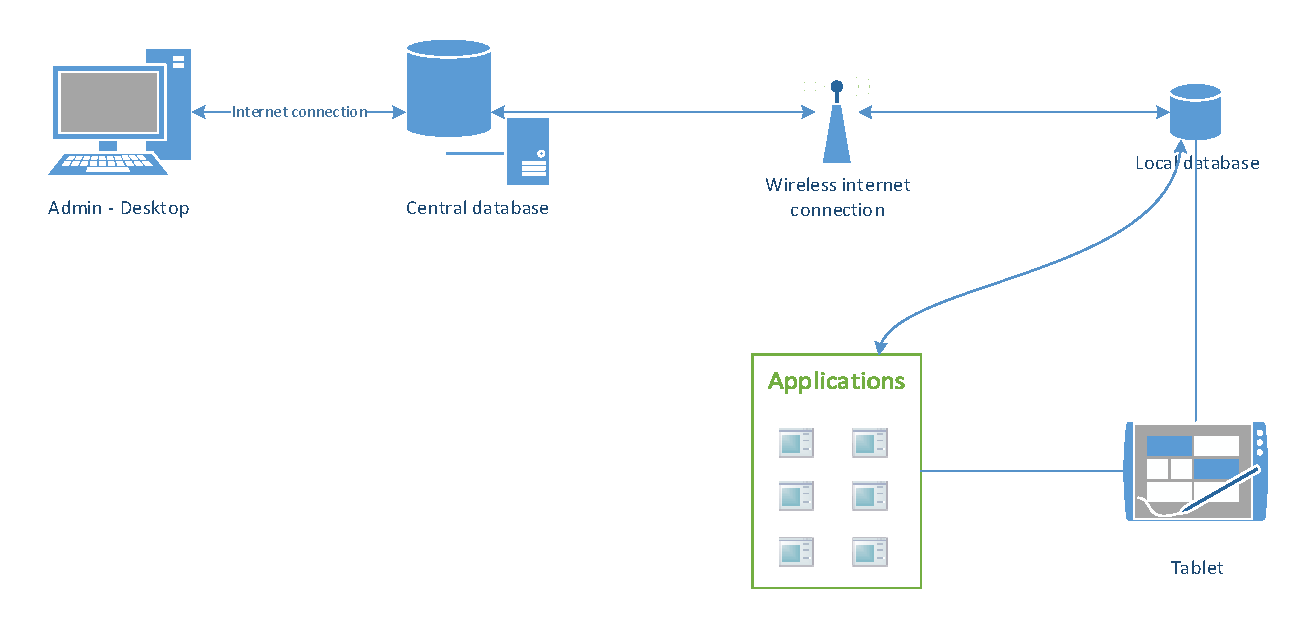
\includegraphics[width=\textwidth]{top_level.pdf}
\label{fig:top_level}
\caption{Top level view of Giraf}
\end{figure}

The applications installed on the tablet are divided into two categories namely games and tools, respectively. The tools provide Giraf with core functionality such as allowing guardians to take pictures with the tablet's onboard camera and add the new picture to one or several children's personal image galleries. They also provide the ability to use pictograms across all applications on the tablet. The games provide some fun learning aids e.g. where the children can learn to control their voice within a game. 

